\chapter{Evaluation\label{evaluation}}

This chapter discusses how the changes implemented in chapter \ref{improvements} impact the performance of RIR.

For evaluation, the Shootout benchmarks were used (see \autocite{shootout} and \autocite{fastr}). These are small programs that focus on different parts of R, such as recursive calls, loops, vector arithmetic, string manipulation etc. The details are in table \ref{tab:shootout}, taken from \autocite{fastr}.

\begin{longtable}[c]{@{}ll@{}}
\caption{The Shootout benchmark suite\label{tab:shootout}} \tabularnewline
\toprule
Benchmark & Description \tabularnewline
\midrule
\endfirsthead
\toprule
Benchmark & Description \tabularnewline
\midrule
\endhead
binarytrees & Allocates and traverses binary trees \tabularnewline
& GC benchmark, recursive calls, recursive lists \tabularnewline
fannkuchred & Solves a combinatorial problem \tabularnewline
& Loops, indexing short vectors \tabularnewline
fasta & Generates DNA sequence by copying, rand. selection \tabularnewline
& String operations, scalar arithmetic \tabularnewline
fastaredux & Solves same problem as fasta \tabularnewline
& Adds more loops, vector indexing and arithmetic \tabularnewline
knucleotide & Finding patterns in gene sequences \tabularnewline
& Uses environment as a hashmap, string operations \tabularnewline
mandelbrot & Calculates a Mandelbrot set (fractal image) \tabularnewline
& Vector arithmetic on complex numbers \tabularnewline
nbody & Solves the N-body problem (simulation) \tabularnewline
& Arithmetic, Math with short vectors \tabularnewline
pidigits & Calculate digits of pi using spigot algorithm \tabularnewline
& Arbitrary precision arithmetic in R (diverse code) \tabularnewline
regexdna & Matching, replacing regex-specified gene sequences \tabularnewline
& Regular expressions (falls back to regex library) \tabularnewline
reversecompl & Computing reverse-complements for gene sequence \tabularnewline
& String vector indexing using string names \tabularnewline
spectralnorm & Computing eigenvalue using power method \tabularnewline
& Loops, function calls, scalar arithmetic \tabularnewline
\bottomrule
\end{longtable}

The benchmarks were run on a machine with \emph{Intel(R) Core(TM) i5-6500} (4 cores) and 8~GB of memory. For every benchmark, three experiments were measured: GNU R interpreted code (JIT set to 0), GNU R byte-compiled code (JIT set to 2 and optimize to 2) and RIR compiled code (JIT set to 2).

Each experiment took place in a fresh R session. The benchmark code was sourced, then it was executed 12 times, and the last 8 measured times were logged. This ensures that the machine is warmed up properly and also disregards any compile time overheads.

The same measurments were performed for every set of added features. The revisions with descriptions that were used to monitor the progress are listed in table \ref{tab:git-rev}.

\begin{longtable}[c]{@{}ll@{}}
\caption{Git revisions used in the benchmarks\label{tab:git-rev}} \tabularnewline
\toprule
Hash & Features \tabularnewline
\midrule
\endfirsthead
\toprule
Hash & Features \tabularnewline
\midrule
\endhead
e1091b9 & State before the first changes \tabularnewline
594af0c & Added relational and unary operators \tabularnewline
ce30085 & Loop contexts removal \tabularnewline
6c4f526 & BC cleanup and colon operator \tabularnewline
f8e8238 & Superassignment operator \tabularnewline
12ef757 & Interpreter loop refactoring \tabularnewline
ff73d75 & Use indirect threading \tabularnewline
\bottomrule
\end{longtable}

Figure \ref{fig:overall} shows the summary of how much the difference between RIR and GNU R was lowered for each benchmark, as well as an overall average. Smaller values are better.

\begin{figure}[htbp]
  \caption{\label{fig:overall}Overview of the slowdown vs. GNU R}
  \centering
  \tmpframe{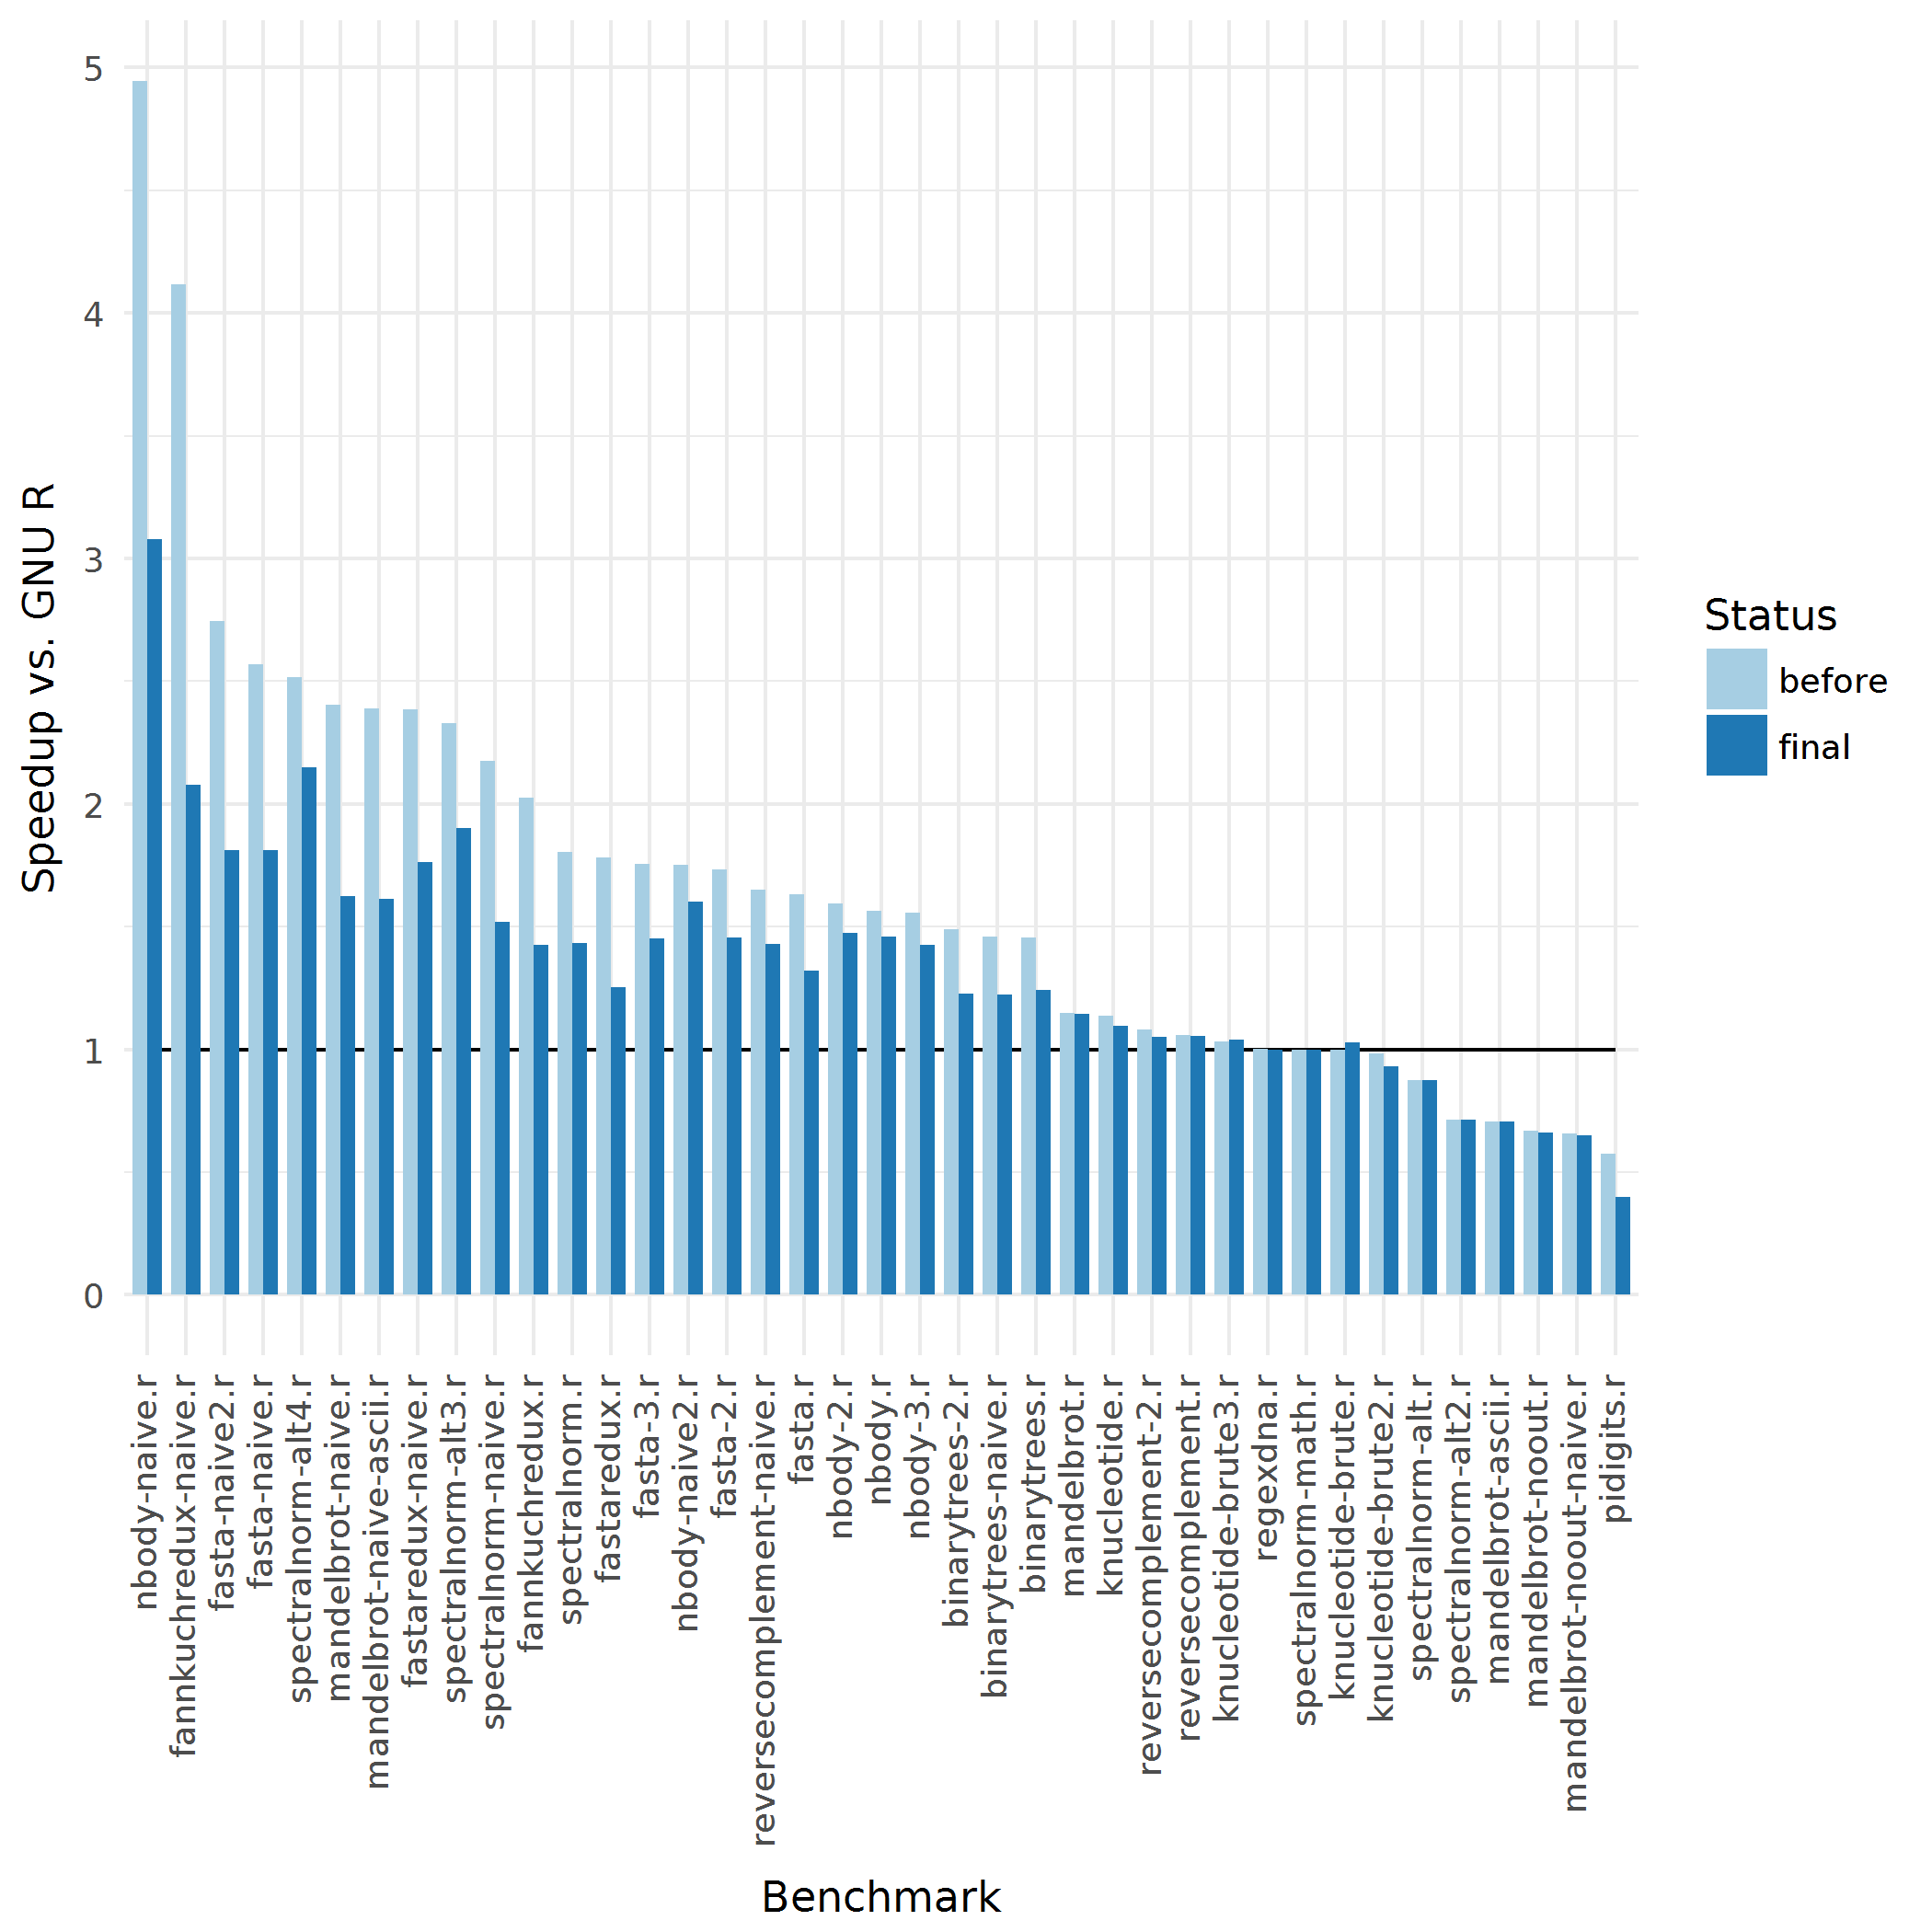
\includegraphics[width=\linewidth]{images/overall}}
\end{figure}

The lighter color refers to the state before anything was done, the darker after all the changes described in chapter \ref{improvements}.

The slowdowns are computed relative to the running time of GNU R byte-compiled code, which was normalized to 1 (this is indicated by the solid black line).

It can be clearly seen that the most speedup was gained in the naive implementations.

Overall, an average slowdown of about 1.678 against GNU R was lowered to about 1.336.

Figure \ref{fig:history} captures the running times of each benchmark over the course of the work described in chapter \ref{improvements}.

\begin{figure}[htbp]
  \caption{\label{fig:history}History of running times}
  \centering
  \tmpframe{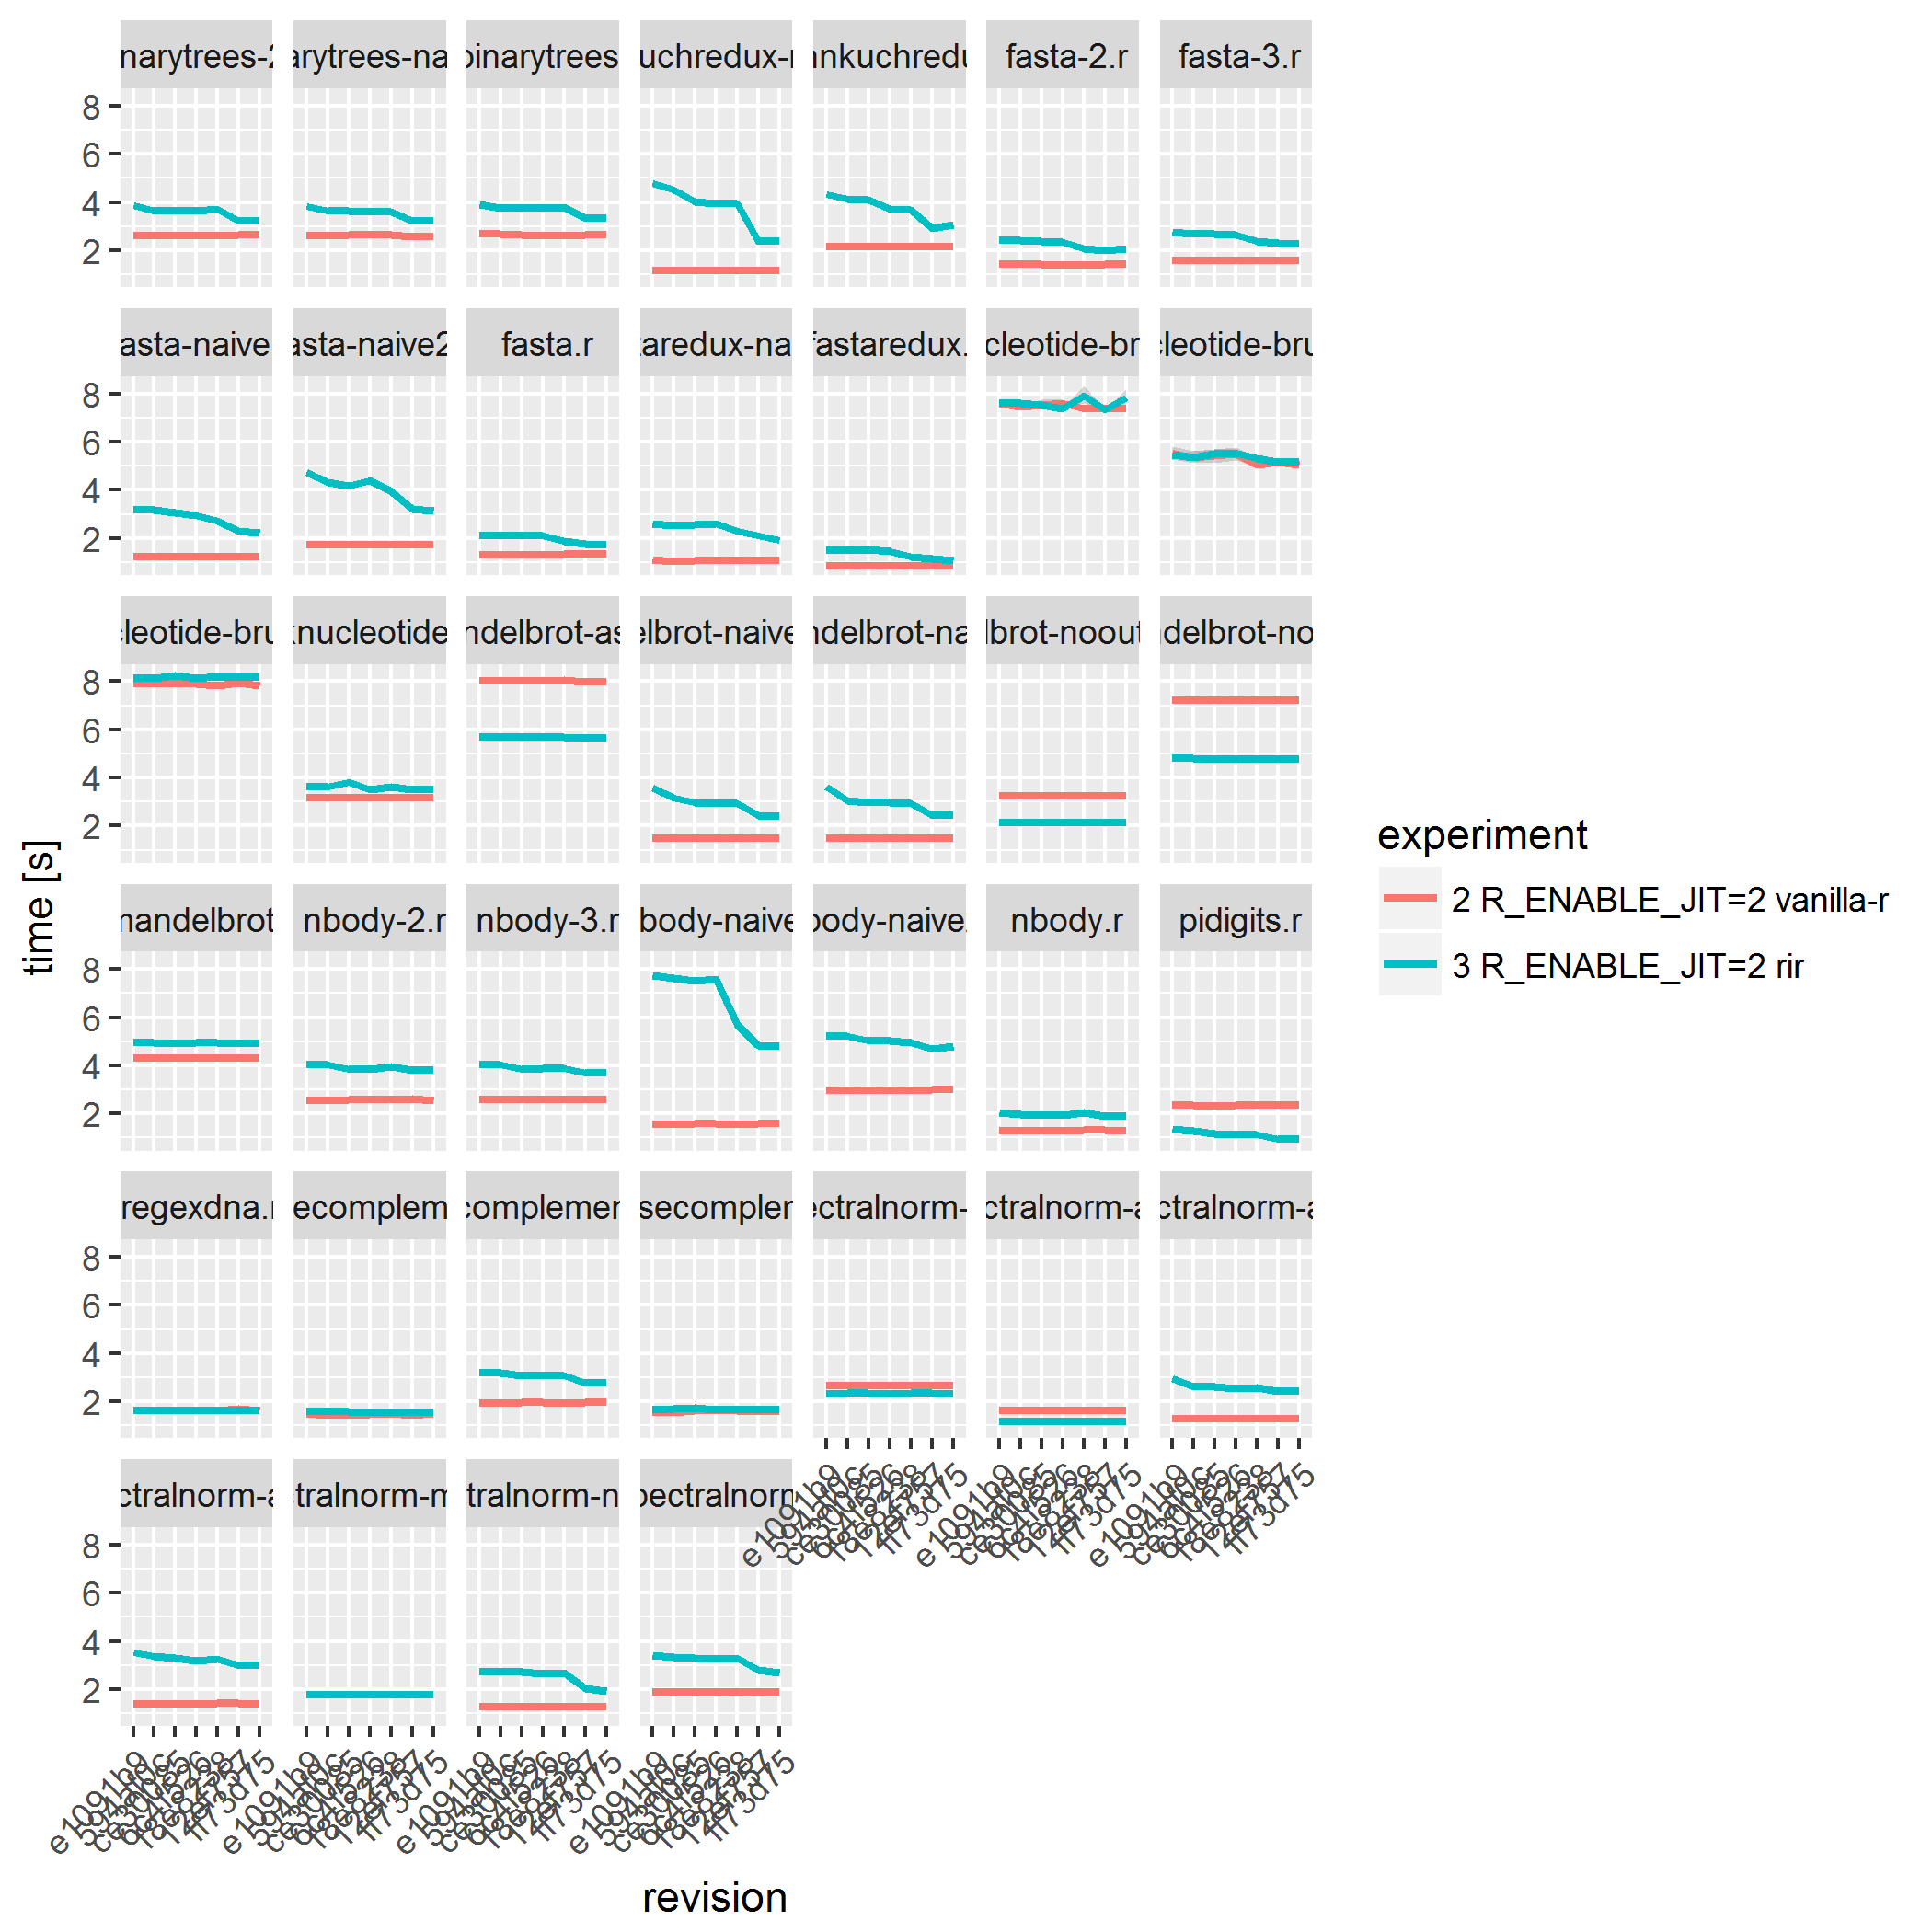
\includegraphics[width=\linewidth]{images/speedup_history}}
\end{figure}

In the figure, the light blue color represents the performance of the GNU R bytecode. As all measurments were carried out on the same version of GNU R (namely 3.3.2) the times are identical.

For three mandelbrot, pidigits and two spectralnorm benchmarks RIR was already faster.

Knucleotide fastanaive some slowdowns.

Some mandelbrot, regexdna, spectralnorm, reversecomplement have not changed at all.

Nbody naive \todo[add plot] big drop interpreter refactoring. also fasta naive, fannkuchrecux naive, spectralnorm naive and others. describe what kind of code they are

\begin{figure}[htbp]
  \caption{\label{fig:}\todo}
  \centering
  \tmpframe{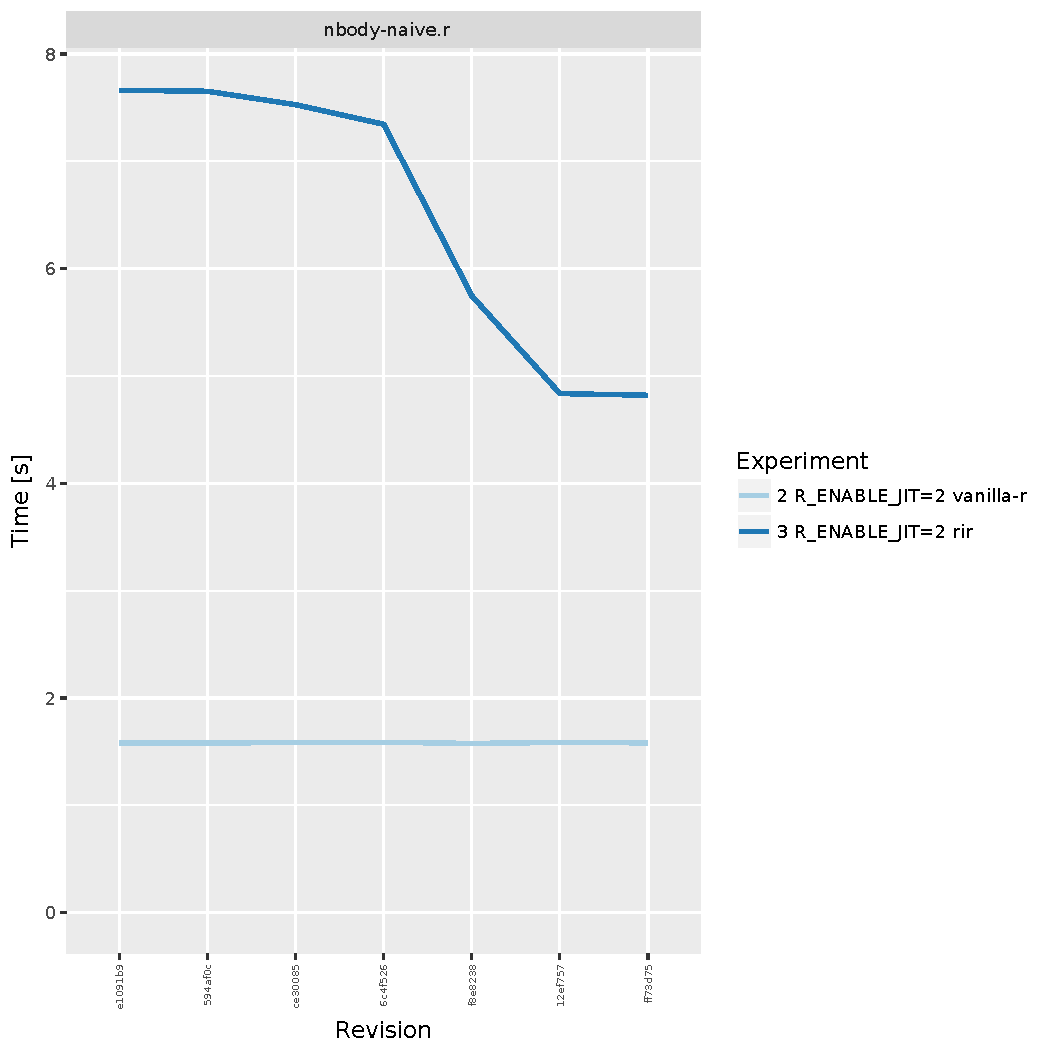
\includegraphics[width=\linewidth]{images/nbody-naive}}
\end{figure}

\begin{figure}[htbp]
  \caption{\label{fig:}\todo}
  \centering
  \tmpframe{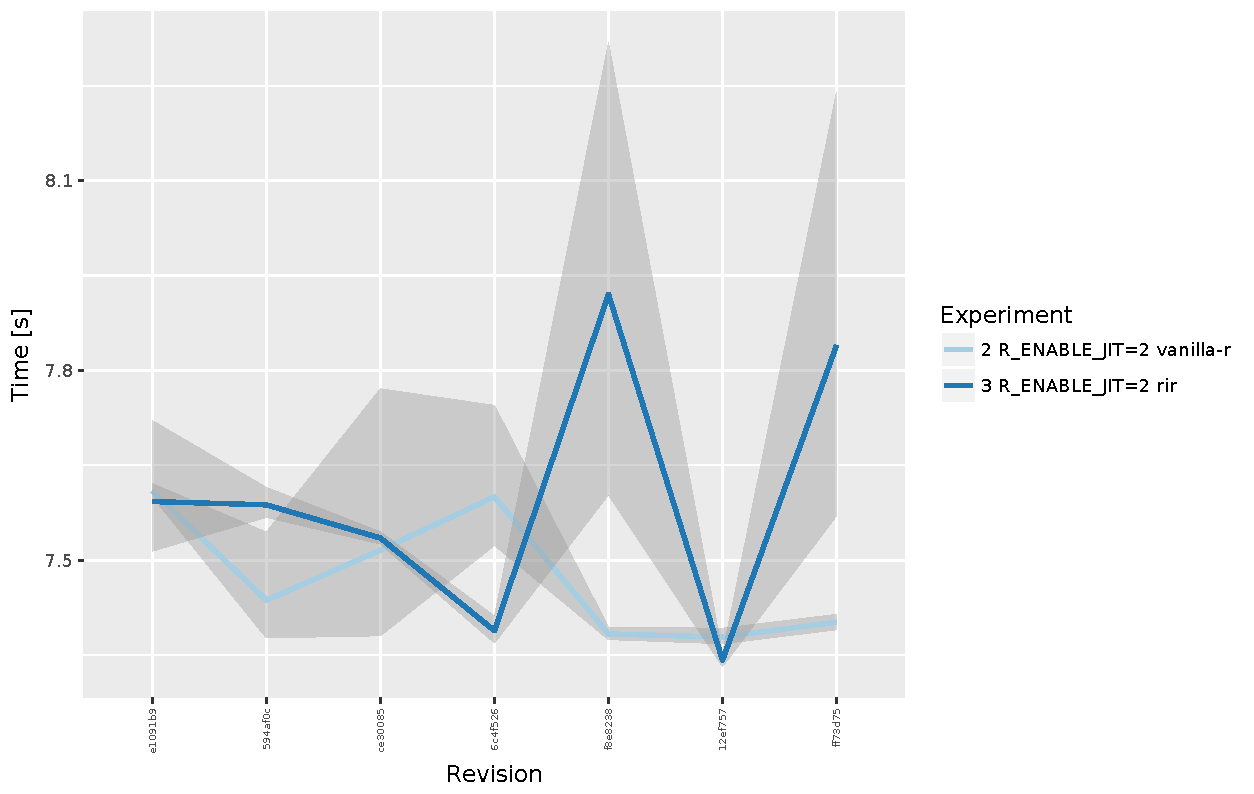
\includegraphics[width=\linewidth]{images/knucleotide-brute}}
\end{figure}

\begin{figure}[htbp]
  \caption{\label{fig:}\todo}
  \centering
  \tmpframe{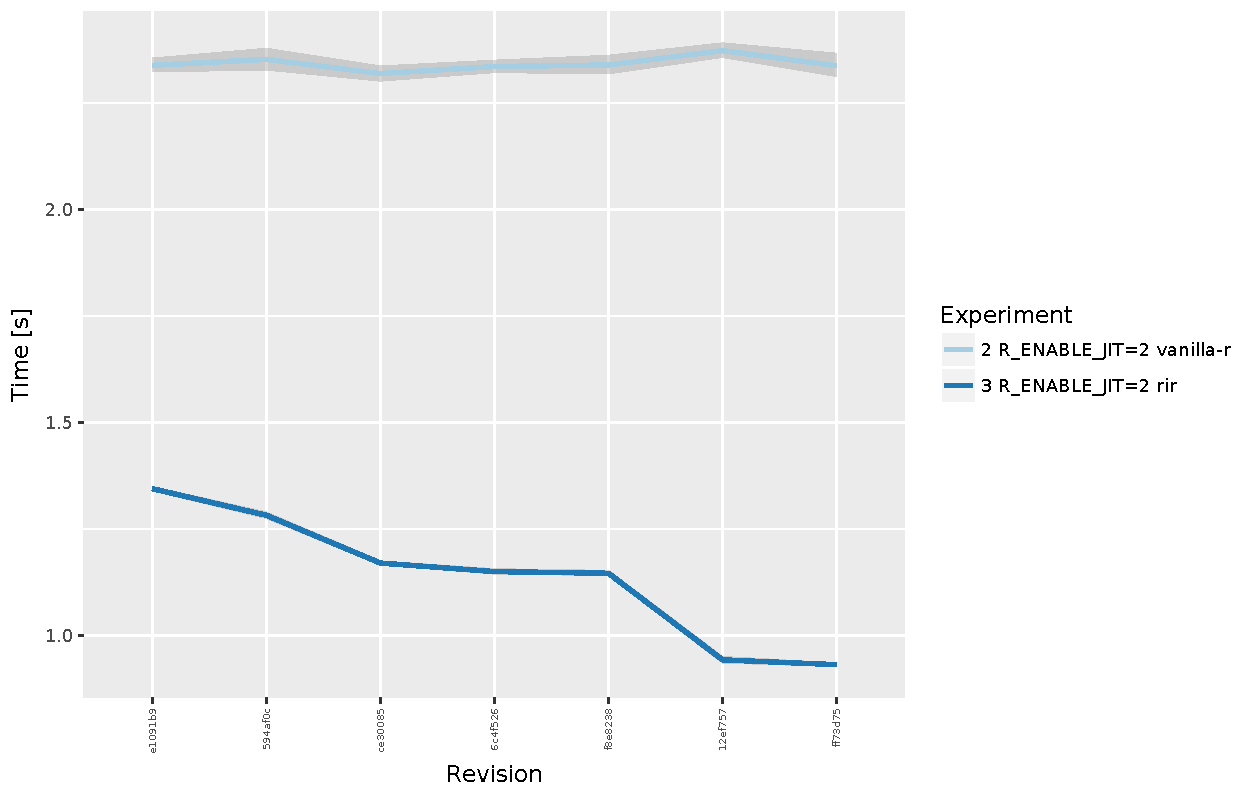
\includegraphics[width=\linewidth]{images/pidigits}}
\end{figure}

Why pidigits so fast and why it improved further

The average speedup versus GNU R over the measured revisions is captured in figure \ref{fig:avg-speedup-history}.

\begin{figure}[htbp]
  \caption{\label{fig:avg-speedup-history}History of average speedup vs. GNU R}
  \centering
  \tmpframe{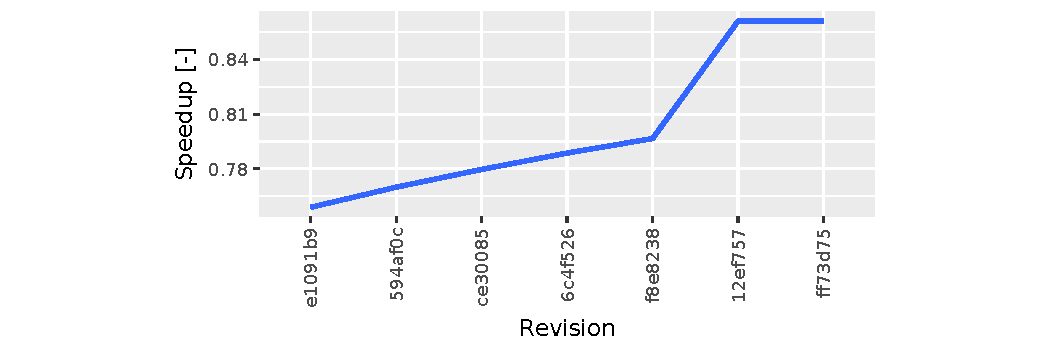
\includegraphics[width=\linewidth]{images/avg_speedup}}
\end{figure}

Additionaly, for ensuring that the improvements had positive effects, usually a kind of microbenchmark, such as the one in listing \ref{lst:microbench}, were checked by hand in fresh sessions of GNU R (with JIT disabled and with JIT set to 2) and RIR (with JIT enabled). In the code, a function is defined and measured repeatedly. The final reported time is computed as arithmetic mean of only a tailing part of the runs. This is to ensure a proper warmup (i.e. everything is byte-compiled by the JIT and possibly the processor branch predictors warm up).

\begin{listing}[htbp]
  \caption{\label{lst:microbench}Microbenchmark code}
  \begin{rcode}
f <- function() {
    i <- 10000000L
    while (i > 0) i <- i - 1
}
t <- c()
for (x in 1:10) t <- c(t, system.time(f())[[3]])
mean(t[5:10])
  \end{rcode}
\end{listing}

In this way, it was for instance found that threaded code starts to pay off only for larger programs.
